
The major contribution of this work is providing a task modeling and setup for learning humanoid soccer movements in the RoboCup Soccer3D domain using reinforcement learning frameworks. We also introduce the deep mimic approach for this class of problems and a specific curriculum to learn, as well as several implementation considerations, manually tunned and developed after a few processes iterations.

\section{Environment and Implementation}

As previously mentioned in section \ref{chap:method}, this work used the RL algorithms implementations from the OpenAI baselines repository \cite{baselines}. More specifically, the high-quality implementation of PPO. Not implementing the DRL algorithms from scratch made it much easier to test, iterate, improve and focus on developing the agent experiments.

The PPO implementation on Baselines was adapted to change the communication with the OpenAI Gym environments to communicate with the Soccer3D agent, maintaining the same function protocols.

The framework used to integrate the baselines code with new experiments, flexible to develop, in the Soccer3D domain was already built in the work \cite{TGMuzio}. This framework can be basically described by its two main modules, each one running as a separate process and communicating through Protocol Buffers.

\begin{itemize}
\item \textbf{Learning Client:} Process that runs the reinforcement learning algorithms and makes remote procedure calls (RPCs) to the server, exchanging state/action information with the soccer agent. This module was implemented in Python 3.5 and TensorFlow, using OpenAI Baselines implementations.

\item \textbf{Soccer Agent:} The simulated agent which interacts with \textit{SimSpark} and with the learning client, executing the learning experiments. This module was implemented in C++ and uses the ITAndroids Soccer Simulation 3D code base.
\end{itemize}

As already commented, the API between server and client uses Protocol Buffers, with the exchange of RPCs containing the standard state, action, reward and end of episode information used in OpenAI Gym. An illustration of this framework follows in the diagram presented in Figure \ref{fig:RL_framework}. For details, please refer to \cite{TGMuzio}.

\begin{figure}[H]
    \centering
    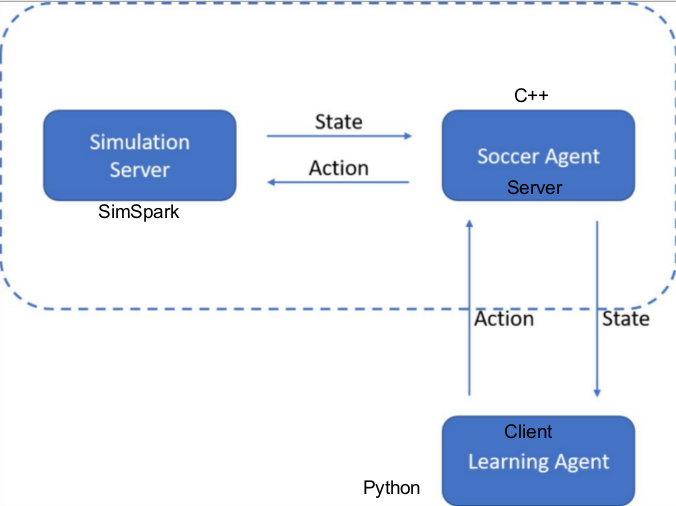
\includegraphics[width=0.8\textwidth]{Chapter6/architecture.png} 
    \caption{Learning Architecture diagram. Extracted from \cite{TGMuzio}}
    \label{fig:RL_framework}
\end{figure}

\section{Infrastructure}

This work used the Intel AI DevCloud as its main infrastructure to run all learning experiments described below.

The cluster is composed by 9 computation nodes using each one a Intel Xeon processor. Furthermore, the experiments setup exploited the parallelization feature of PPO, running up to 12 Soccer Agents per node, besides the Learning Client process, and collecting a total number of samples in the magnitude of 100 million.

\section{Deep Mimic Learning}

The Deep Mimic approach \cite{deepmimic} established a great new paradigm in which this work was based on. It introduces a novel idea of allowing the supply of reference motions from motion capture or hand-authored animation data for style, and then generating goal-directed and physically realistic behavior from those reference motions \cite{deepmimic}.

The basic approach presented for this mission consists in rewarding the agent to produce motions that resemble the reference data, as well as to achieve additional task objectives.

A control policy $\pi (a_t|s_t,g_t)$ maps the state of the character $s_t$ and a task-specific goal $g_t$ to an action $a_t$. The action distribution is gaussian, with fixed covariance and mean given by a neural network. This policy outputs the desired joints positions, which is later translated into torque commands by each joint PD controller.

The overall reward is spitted into the imitation reward, given by $r_I(s_t,a_t)$, and the task-specific reward, given by $r_G(s_t,a_t)$. The final reward is therefore given by Equation \ref{eq:deep_mimic_reward}.

\begin{equation}
r_t = \omega^I r_t^I + \omega^G r_t^G
\label{eq:deep_mimic_reward}
\end{equation}

The policies are trained with PPO using the clipped surrogate objective, maintaining also a further network for the value function $V_{\psi}(s,g)$.

It is worth mentioning that this work introduces also two novel ideas which significantly increased the robustness and performance of the learning behaviors. 

\begin{itemize}
\item \textit{Reference State Initialization} (RSI) randomly selects a state in which the agent ant its reference actor begins at each episode. In this way, it makes possible to discover high reward future states without the need to learn everything until then, which can be very significant in difficult tasks as backflips.

\item \textit{Early Termination} (ET) finishes the episode when the agent reaches any fruitless condition, such as a fall or joints collision. This process discourage undesirable behaviors and the exploration of bad states, therefore increasing the learning efficiency.
\end{itemize}

\section{Pure Mimic Task}

\section{Fixed Final Distance Task}




